\section{地磁场}\label{sec:10-3}

\begin{wrapfigure}{r}{7cm}
    \centering
    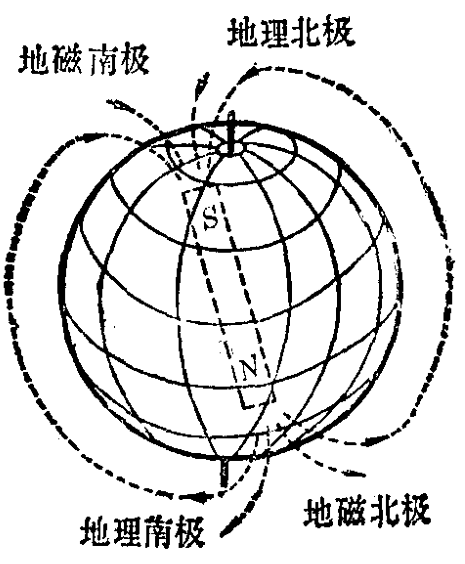
\includegraphics[width=6cm]{../pic/czwl2-ch10-13}
    \caption{地磁场}\label{fig:10-13}
\end{wrapfigure}

我们已经知道,一个能在水平面内自由转动的磁针,静止时总是一端指南,一端指北。
这是为什么呢?原来,地球本身是一个巨大的磁体。
地磁的北极在地理南极附近,地磁的南极在地理北极附近。
因此,在地球周围的空间里存在着磁场,这个磁场叫做\textbf{地磁场}。
磁针静止时总是一端指南,一端指北,就是因为受到了地磁场的作用。
由于\CJKunderwave{地理两极跟地磁两极并不重合}(图 \ref{fig:10-13}),
因此,水平放置的磁计的指向,跟地理子午线并不一致,其间有一交角,叫做磁偏角。

我国宋代的科学家沈括(1031 ~ 1095)是世界上第一个清楚地、准确地论述磁偏角的科学家。
他明确指出,指南针所指方向经常是稍微偏离南北方向的。
这比西方哥仑布横渡大西洋时(1492 年)才观察到地磁偏角的现象早了四百多年。

地磁场是怎么产生的?这个问题已经研究了多年,但是直到现在还没有得到满意的结果。


\lianxi

(1) 当钢条靠近磁针的磁极时,磁极自动接近钢条,能不能根据这一现象确定钢条具有磁性?
为什么?如果磁极躲开钢条呢?

(2) 一块磁铁我们不知道它的哪端是南极,哪端是北极,怎样才能判别?你能想出几种办法?

(3) 有两根外形完全相同的钢棒,一根有磁性,另一根没有磁性,
如果没有任何其他用具,怎样才能知道哪一根有磁性,哪一根没有磁性?


(4) 磁铁旁小磁针静止时所指的方向如图 \ref{fig:10-14} 所示,画出磁力线的方向,
并标出磁铁的 $N$、$S$ 极。(小磁针黑端是 $N$ 极)

\begin{figure}[htbp]
    \centering
    \begin{minipage}{10cm}
    \centering
    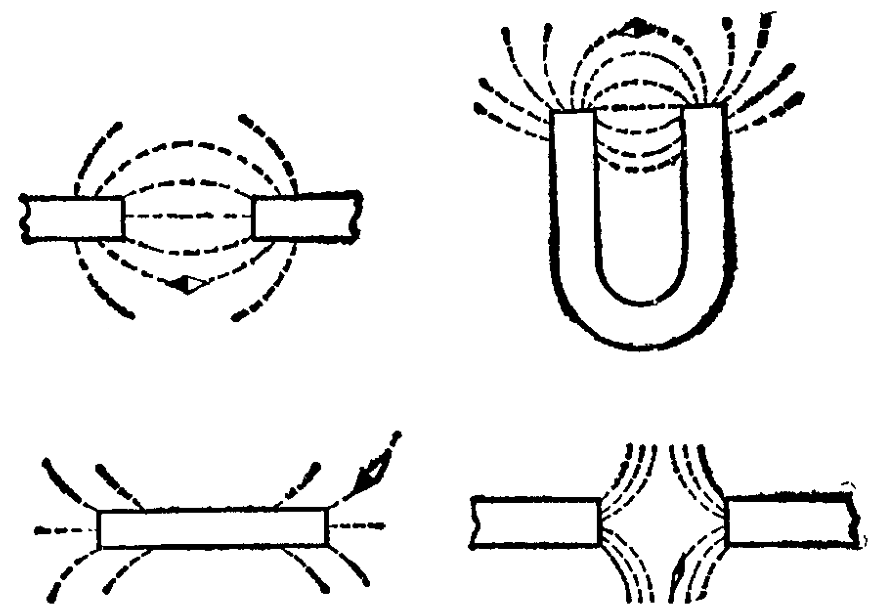
\includegraphics[width=10cm]{../pic/czwl2-ch10-14}
    \caption{}\label{fig:10-14}
    \end{minipage}
    \qquad
    \begin{minipage}{5cm}
    \centering
    \vspace{5cm}
    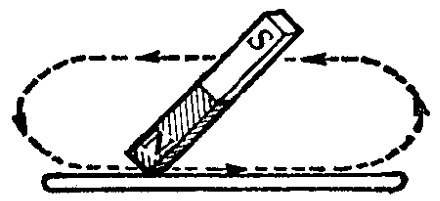
\includegraphics[width=5cm]{../pic/czwl2-ch10-15}
    \caption{}\label{fig:10-15}
    \end{minipage}
\end{figure}

(5) 用磁铁的一极在一根钢棒上沿同一方向摩擦几次(图 \ref{fig:10-15}),钢棒就被磁化了,
用它可以吸起铁屑、大头针等。钢铁做的任何小东西,如钢锯条、钢尺、小刀、缝衣针等都可以用这种方法来磁化。
试用上述方法将身边的小形钢铁物体磁化,并用它来吸引别的轻小钢铁制品。

